% messydates cheat sheet — editable source
% Build:  pdflatex cheatsheet.tex   (run from this directory)
% See build.R in this folder to compile and refresh the PDF/PNG copies.
\documentclass[9pt]{extarticle}

\usepackage[paperwidth=11in,paperheight=7.6in,margin=0.4in]{geometry}
\usepackage[T1]{fontenc}
\usepackage{helvet}
\renewcommand{\familydefault}{\sfdefault}
\usepackage{inconsolata}
\usepackage{graphicx}
\usepackage{xcolor}
\usepackage{multicol}
\usepackage{array}
\usepackage[most]{tcolorbox}
\usepackage{fontawesome5}
\usepackage{tikz}
\usepackage{enumitem}
\setlist[itemize]{leftmargin=1.15em, itemsep=1pt, topsep=1pt, parsep=0pt}

\graphicspath{{../../man/figures/}}
\pagestyle{empty}
\setlength{\parindent}{0pt}

% --- palette (matches the wooden/sundial theme) ---
\definecolor{mdtan}{HTML}{E9D8B4}
\definecolor{mddark}{HTML}{B58B4C}
\definecolor{mdbrown}{HTML}{6E5334}
\definecolor{mdgrey}{HTML}{E7E7E7}
\definecolor{mdgreyd}{HTML}{8A8A8A}
\definecolor{mdink}{HTML}{2B2016}

% inline verbatim code (no escaping needed): \code|as_messydate(x)|
\let\code\verb

% --- section boxes ---
\newtcolorbox{mdbox}[2][mddark]{
  enhanced, breakable=false,
  colback=mdtan!22, colframe=#1, coltitle=white,
  colbacktitle=#1, fonttitle=\bfseries,
  title={#2}, boxrule=0.5pt, arc=2pt,
  left=3pt, right=3pt, top=2pt, bottom=3pt,
  before skip=6pt, after skip=6pt,
  fontupper=\small
}
\newtcolorbox{greybox}[1]{
  enhanced, breakable=false,
  colback=mdgrey, colframe=mdgreyd, coltitle=white,
  colbacktitle=mdgreyd, fonttitle=\bfseries,
  title={#1}, boxrule=0.5pt, arc=2pt,
  left=3pt, right=3pt, top=2pt, bottom=3pt,
  before skip=6pt, after skip=6pt,
  fontupper=\small
}
\newcommand{\arrow}{\;\textcolor{mddark}{$\rightarrow$}\;}

\begin{document}

% ======================= HEADER =======================
\begin{tcolorbox}[enhanced, colback=mdbrown, colframe=mdbrown, arc=3pt,
  left=8pt, right=8pt, top=4pt, bottom=4pt]
\begin{minipage}[c]{0.80\textwidth}
  {\color{white}\bfseries\fontsize{22}{24}\selectfont
   Arrange your messy dates \& times \; : : \; CHEAT SHEET}\\[2pt]
  {\color{mdtan}\small Retain, represent, and reason about date/time
   imprecision — an implementation of ISO 8601-2:2019 (EDTF) for R.}
\end{minipage}\hfill
\begin{minipage}[c]{0.16\textwidth}\raggedleft
  
\includegraphics[height=1.05in]{messydates_hexlogo.png}
\end{minipage}
\end{tcolorbox}

\vspace{2pt}
\setlength{\columnsep}{9pt}
\begin{multicols}{3}

% ------------- BASICS / ANNOTATIONS -------------
\begin{greybox}{Basics: annotate dates \& times}
The \code|mdate| class embeds EDTF annotations, so one value can express
imprecision instead of forcing a false precise date:

\smallskip
\renewcommand{\arraystretch}{1.25}
\begin{tabular}{@{}p{1.05cm}l@{}}
\code|?|  & uncertain \quad\code|2008-01-18?|\\
\code|~|  & approximate \quad\code|2012-09-12~|\\
\code|%|  & uncertain \& approximate\\
\code|X|  & unspecified \quad\code|2012-XX-18|\\
\code|..| & range \quad\code|2012-01..2012-03|\\
\code|{} []| & set (all) / one-of\\
\code|T|  & time + zone \quad\code|...T14:30Z|\\
\end{tabular}
\end{greybox}

% ------------- 1. COERCE -------------
\begin{mdbox}{1. Coerce objects to \texttt{mdate}}
\code|as_messydate(x)| coerces \code|Date|, \code|POSIXct|, \code|POSIXlt|,
character, or written text (dates \emph{and} times) into \code|mdate|:

\smallskip
\renewcommand{\arraystretch}{1.2}
\begin{tabular}{@{}ll@{}}
\textbf{input} & \textbf{mdate}\\ \hline
\code|"2021-04"|            & \code|2021-04|\\
\code|"2012-09-12~"|        & \code|2012-09-12~|\\
\code|"2012-01..2012-03"|   & \code|2012-01..2012-03|\\
\code|"first of Feb 2012"|  & \code|2012-02-01|\\
\code|"2019-03-01 2:30pm"|  & \code|2019-03-01T14:30|\\
\end{tabular}

\smallskip
\code|make_messydate(year, month, day)| builds from columns:
\code|(2007, 2, 17)| \arrow \code|2007-02-17|.
\end{mdbox}

% ------------- 2. EXPAND / CONTRACT -------------
\begin{mdbox}{2. Expand \& contract}
\code|expand(md)| opens a messy date into \emph{all} compatible dates
(day granularity; use \code|by="hour"/"min"/"sec"| for times):
\begin{itemize}
  \item \code|"2021-04"| \arrow 30 dates \code|2021-04-01 ... -04-30|
  \item \code|"2019-02-01..2019-02-03"| \arrow 3 dates
\end{itemize}
\code|contract(md)| is the inverse — the most concise form:
\code|"2021-04-01..2021-04-30"| \arrow \code|2021-04|.
\end{mdbox}

% ------------- 3. RESOLVE -------------
\begin{mdbox}{3. Resolve to one date/time}
Coerce back with \code|as.Date()|, \code|as.POSIXct()|, or \code|as.POSIXlt()|
(the POSIX methods keep the time). Choose \emph{how} to resolve with
\code|FUN =|:
\smallskip

\code|min max mean median modal random| (whole vector), or vectorised
\code|vmin vmax vmean vmedian vmodal vrandom| (element-wise).
\smallskip

\code|as.Date(as_messydate("2021-04"), vmin)| \arrow \code|2021-04-01|\\
\code|                          ..., vmax)| \arrow \code|2021-04-30|\\
\code|                          ..., vmean)| \arrow \code|2021-04-16|

\smallskip
\begin{center}
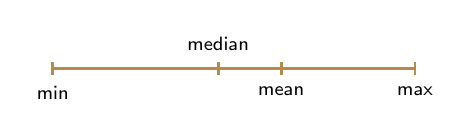
\begin{tikzpicture}
\draw[mddark, line width=1pt] (0,0) -- (4.6,0);
\foreach \x in {0, 2.1, 2.9, 4.6}
  \draw[mddark, line width=1pt] (\x,-2.5pt) -- (\x,2.5pt);
\node[below, font=\scriptsize] at (0,-3pt){min};
\node[above, font=\scriptsize] at (2.1,3pt){median};
\node[below, font=\scriptsize] at (2.9,-3pt){mean};
\node[below, font=\scriptsize] at (4.6,-3pt){max};
\end{tikzpicture}
\end{center}
\end{mdbox}

% ------------- TIMES -------------
\begin{mdbox}[mdbrown]{\faClock\; Times (new in 1.0.0)}
Times of day use the ISO \code|T| separator, and take the same
annotations as dates:
\begin{itemize}
  \item \textbf{Parse:} \code|"2019-03-01T14:30:00Z"|, am/pm,
        \code|+02:00| offsets, fractional seconds.
  \item \textbf{Extract:} \code|hour() minute() second() tz()|.
  \item \textbf{Annotate a part:} \code|as_approximate(x,"hour")|
        \arrow \code|...T~14:30|.
  \item \textbf{Precision below a day:} \code|precision("...T14:30")|=1440
        (\code|24| hr, \code|1440| min, \code|86400| sec).
  \item \textbf{Shift \& step:} \code|md + "2 hours"|;
        \code|seq(a, b, by="hour")|.
\end{itemize}
\end{mdbox}

% ------------- ANNOTATE -------------
\begin{mdbox}{Annotate uncertainty}
\renewcommand{\arraystretch}{1.2}
\begin{tabular}{@{}ll@{}}
\code|on_or_before(x)|   & \arrow \code|..x|\\
\code|on_or_after(x)|    & \arrow \code|x..|\\
\code|as_approximate(x)| & \arrow \code|x~|\\
\code|as_uncertain(x)|   & \arrow \code|x?|\\
\end{tabular}\\[2pt]
Add \code|component=| to mark one part: \code|"year" "month" "day"|
\code|"hour" "minute" "second"|, or groups \code|"ym" "md" "time"|.
\end{mdbox}

% ------------- COMBINE -------------
\begin{mdbox}{Combine two mdates}
\begin{itemize}
  \item \code|x %intersect% y| — dates common to both
  \item \code|x %union% y| — dates in either
  \item \code|x + y| — multiset (union of ranges/sets)
\end{itemize}
\end{mdbox}

% ------------- TEST -------------
\begin{mdbox}{Logical tests}
\code|is_messydate(x)| \code|is_precise(x)| \code|is_uncertain(x)|
\code|is_approximate(x)| \code|is_bce(x)|\\[2pt]
\code|is_intersecting(x,y)| \code|is_subset(x,y)| \code|is_similar(x,y)|
\end{mdbox}

% ------------- COMPARE -------------
\begin{mdbox}{Proportional comparison}
Proportion of \code|x|'s possible dates meeting a test against \code|y|:
\begin{itemize}
  \item \code|x %l% y| before min \hfill \code|x %le% y| $\le$
  \item \code|x %g% y| after max \hfill \code|x %ge% y| $\ge$
  \item \code|x %><% y| within \hfill \code|x %>=<% y| within, incl.
\end{itemize}
\end{mdbox}

% ------------- COMPONENTS / DURATION -------------
\begin{mdbox}{Components \& durations}
Extract \code|year() month() day() hour() minute() second() tz()|,
or measure \code|precision()|.\\[2pt]
\code|messyduration(range)| returns a duration that accounts for the
uncertainty at each end.
\end{mdbox}

\end{multicols}

\vfill
{\scriptsize\color{mdink}
MIT License \copyright\ 2021--2026 \; \textbullet\; www.panarchic.ch \; \textbullet\;
Learn more at \textbf{https://globalgov.github.io/messydates/} \; \textbullet\;
package version 1.0.0 \; \textbullet\; Updated: 2026-07}

\end{document}
